\begin{figure}[t]
  \vspace{-1.0em}
  \centering
  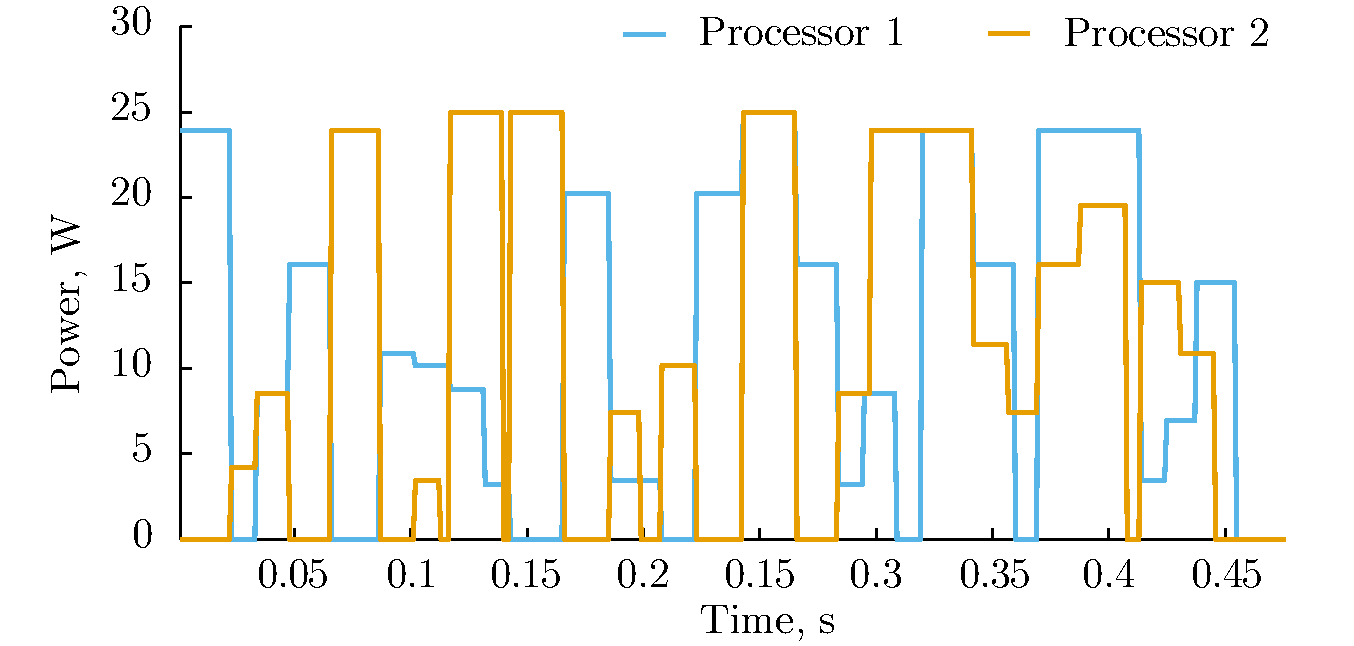
\includegraphics[width=0.90\columnwidth]{include/assets/application-power.pdf}
  \caption{A dynamic power profile.}
  \flabel{power}
  \vspace{-1.5em}
\end{figure}

\begin{figure}
  \centering
  \updatedFigure{
  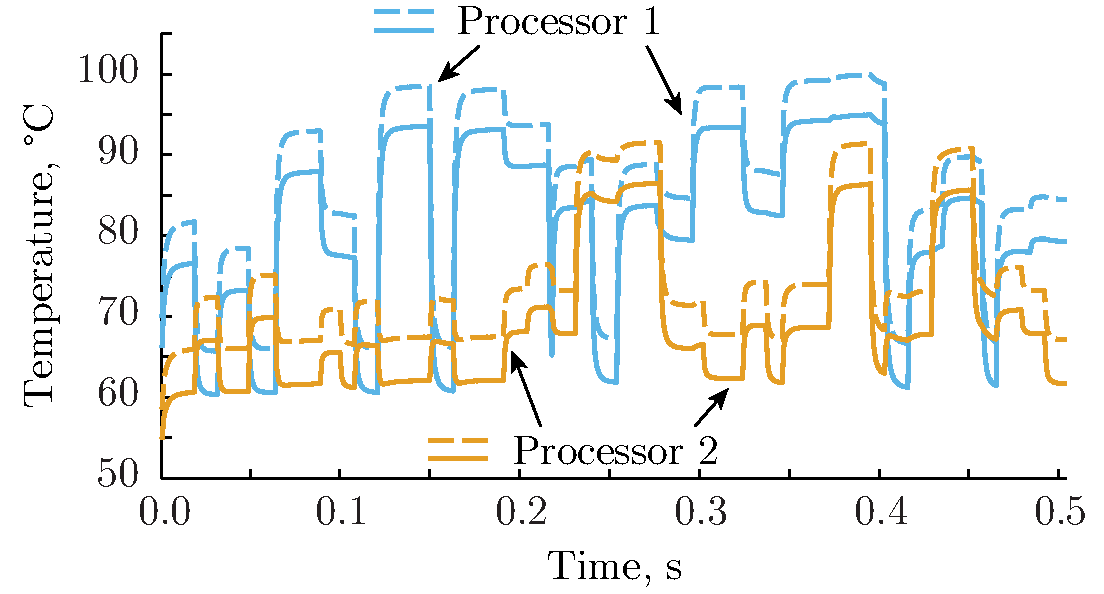
\includegraphics[width=0.90\columnwidth]{include/assets/application-temperature.pdf}
  }
  \vspace{-1.0em}
  \caption{The expected temperature (the solid lines) and one standard deviation above it (the dashed lines).}
  \flabel{application-temperature}
  \vspace{-1.0em}
\end{figure}

We turn to \stage{5}\ in \fref{algorithm}.
It can be seen in, for example, \eref{pc-example} that the surrogate model has a negligibly small computational cost at this stage: for any outcome of the uncertain parameters $\vZ(\o) \equiv \vZ$, we can easily compute the corresponding temperature by plugging in $\vZ$ into \eref{pc-example}; the same applies for power.
Consequently, the constructed representation can be trivially analyzed to retrieve various statistics of the system in \eref{fourier-system}.
Let us illustrate a few of them still retaining the example given in \eref{pc-example}.
Assume that the dynamic power profile, $\profilePdyn$, corresponding to the considered workload is the one shown in \fref{application-power}.
Having constructed the surrogate with respect to this profile, we can then rigorously estimate, say, the \pdf\ of temperature at some $k$th moment of time by sampling the surrogate and obtain curves similar to those shown \fref{experimental-results-pdf} (to be discussed in \sref{experimental-results}).
Furthermore, the expectation and variance of temperature are calculated as simply as (see \eref{pc-moments})
\[
  \oExp{\vTO_k(\o)} = \pcc{\vTO}_{k1} \hspace{1em} \text{and} \hspace{1em} \oVar{\vTO_k(\o)} = \sum_{i = 2}^{6} \pcn_i \: \pcc{\vTO}_{ki}^2
\]
where $\pcn_i$ are normalization constants, and the squaring should be understood element-wise.
For the whole time span of the power profile $\profilePdyn$ depicted in \fref{application-power}, these quantities are plotted in \fref{application-temperature}.
The displayed curves closely match those obtained via MC simulations with $10^4$ samples; however, our method takes less than a second whilst MC sampling takes more than a day as we shall see next.
